\documentclass{bioinfo}
\copyrightyear{2016} \pubyear{2016}

%% Some pieces required from the pandoc template
\providecommand{\tightlist}{%
  \setlength{\itemsep}{0pt}\setlength{\parskip}{0pt}}


% Pandoc citation processing


% hyperref makes the margins screwy.
% https://groups.google.com/forum/#!topic/latexusersgroup/4W_SwGk6zx4
% http://ansuz.sooke.bc.ca/software/latex-tricks.php
% \usepackage[colorlinks=true, allcolors=blue]{hyperref}

\access{Advance Access Publication Date:   }
\appnotes{Manuscript Category}

\begin{document}
\firstpage{1}

\subtitle{Application Note}

\title[JBrowseR: R Interface to JBrowse 2]{JBrowseR: An R Interface to
the JBrowse 2 Genome Browser}

\author[FirstAuthorLastName \textit{et~al}.]{
Elliot Hershberg\,\textsuperscript{1},
Garrett Stevens\,\textsuperscript{1},
Colin Diesh\,\textsuperscript{1},
Peter Xie\,\textsuperscript{1},
Teresa De Jesus Martinez\,\textsuperscript{1},
Rob Buels\,\textsuperscript{1},
Lincoln Stein\,\textsuperscript{2},
Ian Holmes\,\textsuperscript{1*},
}

\address{
\textsuperscript{1}Department of Bioengineering, University of
California, Berkeley, Berkeley, CA 94720, USA\\
\textsuperscript{2}Ontario Institute for Cancer Research, Toronto, ON
M5G 0A3, Canada\\
}

\corresp{*To whom correspondence should be addressed. E-mail:
ihh@berkeley.edu}

\history{Received on XXX; revised on XXX; accepted on XXX}

\editor{Associate Editor: XXX}

\abstract{
\textbf{Motivation:} Genome browsers are an essential tool in genome
analysis. Modern genome browsers enable complex and interactive
visualization of a wide variety of genomic data modalities. While such
browsers are very powerful, they can be challenging to configure and
program for bioinformaticians lacking expertise in web development.\\
\textbf{Results:} We have developed an R package that provides an
interface to the JBrowse 2 genome browser. The package can be used to
configure and customize the browser entirely with R code. The browser
can be deployed from the R console, or embedded in Shiny applications or
R Markdown documents.\\
\textbf{Availability:} JBrowseR is available for download from CRAN, and
the source code is openly available from the Github repository at\\
\textbf{Contact:}ihh@berkeley.edu\\
\textbf{Supplementary information:} Supplementary data are available at
Bioinformatics Online.}

\maketitle

\section{Introduction}

Cite others using bracket notation \citep{pepe2003statistical}. Can also
cite with \citet{zou2005regularization}.

Instructions for authors are available
\href{http://www.oxfordjournals.org/our_journals/bioinformatics/for_authors/general.html}{online}.

Introduce your topic. Lorem ipsum ad nauseum. Introduce your topic.
Lorem ipsum ad nauseum. Introduce your topic. Lorem ipsum ad nauseum.
Introduce your topic. Lorem ipsum ad nauseum. Introduce your topic.
Lorem ipsum ad nauseum.

Introduce your topic. Lorem ipsum ad nauseum. Introduce your topic.
Lorem ipsum ad nauseum. Introduce your topic. Lorem ipsum ad nauseum.
Introduce your topic. Lorem ipsum ad nauseum. Introduce your topic.
Lorem ipsum ad nauseum.

\section{Approach}

Here is how to include math equations in the document (bounded by
\texttt{\$\$}):

\[
\begin{aligned}
(x+y)^3&=(x+y)(x+y)^2\\
       &=(x+y)(x^2+2xy+y^2) \label{eqn:example} \\
       &=x^3+3x^2y+3xy^3+x^3. 
\end{aligned}
\]

Describe the approach. Lorem ipsum ad nauseum. Introduce your topic.
Lorem ipsum ad nauseum. Introduce your topic. Lorem ipsum ad nauseum.
Introduce your topic. Lorem ipsum ad nauseum. Introduce your topic.
Lorem ipsum ad nauseum.

Describe the approach. Lorem ipsum ad nauseum. Introduce your topic.
Lorem ipsum ad nauseum. Introduce your topic. Lorem ipsum ad nauseum.
Introduce your topic. Lorem ipsum ad nauseum. Introduce your topic.
Lorem ipsum ad nauseum.

Describe the approach. Lorem ipsum ad nauseum. Introduce your topic.
Lorem ipsum ad nauseum. Introduce your topic. Lorem ipsum ad nauseum.
Introduce your topic. Lorem ipsum ad nauseum. Introduce your topic.
Lorem ipsum ad nauseum.

Describe the approach. Lorem ipsum ad nauseum. Introduce your topic.
Lorem ipsum ad nauseum. Introduce your topic. Lorem ipsum ad nauseum.
Introduce your topic. Lorem ipsum ad nauseum. Introduce your topic.
Lorem ipsum ad nauseum.

\begin{figure}
\centering
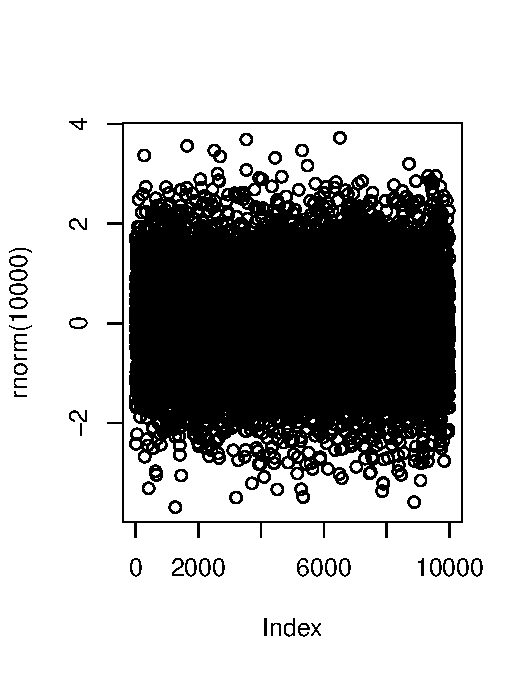
\includegraphics{JBrowseR-paper_files/figure-latex/figure-1.pdf}
\caption{Figure from an Rmd chunk.}
\end{figure}

\section{Methods}

Detailed methods. Lorem ipsum ad nauseum. Introduce your topic. Lorem
ipsum ad nauseum. Introduce your topic. Lorem ipsum ad nauseum.
Introduce your topic. Lorem ipsum ad nauseum. Introduce your topic.
Lorem ipsum ad nauseum.

Detailed methods. Lorem ipsum ad nauseum. Introduce your topic. Lorem
ipsum ad nauseum. Introduce your topic. Lorem ipsum ad nauseum.
Introduce your topic. Lorem ipsum ad nauseum. Introduce your topic.
Lorem ipsum ad nauseum.

Detailed methods. Lorem ipsum ad nauseum. Introduce your topic. Lorem
ipsum ad nauseum. Introduce your topic. Lorem ipsum ad nauseum.
Introduce your topic. Lorem ipsum ad nauseum. Introduce your topic.
Lorem ipsum ad nauseum.

\subsection{Sub-Method}

Details for Method 1. Lorem ipsum ad nauseum. Introduce your topic.
Lorem ipsum ad nauseum. Introduce your topic. Lorem ipsum ad nauseum.
Introduce your topic. Lorem ipsum ad nauseum. Introduce your topic.
Lorem ipsum ad nauseum.

Details for Method 1. Lorem ipsum ad nauseum. Introduce your topic.
Lorem ipsum ad nauseum. Introduce your topic. Lorem ipsum ad nauseum.
Introduce your topic. Lorem ipsum ad nauseum. Introduce your topic.
Lorem ipsum ad nauseum.

Details for Method 1. Lorem ipsum ad nauseum. Introduce your topic.
Lorem ipsum ad nauseum. Introduce your topic. Lorem ipsum ad nauseum.
Introduce your topic. Lorem ipsum ad nauseum. Introduce your topic.
Lorem ipsum ad nauseum.

Details for Method 1. Lorem ipsum ad nauseum. Introduce your topic.
Lorem ipsum ad nauseum. Introduce your topic. Lorem ipsum ad nauseum.
Introduce your topic. Lorem ipsum ad nauseum. Introduce your topic.
Lorem ipsum ad nauseum.

\subsection{Method 2}

Details for Method 2. Lorem ipsum ad nauseum. Introduce your topic.
Lorem ipsum ad nauseum. Introduce your topic. Lorem ipsum ad nauseum.
Introduce your topic. Lorem ipsum ad nauseum. Introduce your topic.
Lorem ipsum ad nauseum.

Details for Method 2. Lorem ipsum ad nauseum. Introduce your topic.
Lorem ipsum ad nauseum. Introduce your topic. Lorem ipsum ad nauseum.
Introduce your topic. Lorem ipsum ad nauseum. Introduce your topic.
Lorem ipsum ad nauseum.

Details for Method 2. Lorem ipsum ad nauseum. Introduce your topic.
Lorem ipsum ad nauseum. Introduce your topic. Lorem ipsum ad nauseum.
Introduce your topic. Lorem ipsum ad nauseum. Introduce your topic.
Lorem ipsum ad nauseum.

Details for Method 2. Lorem ipsum ad nauseum. Introduce your topic.
Lorem ipsum ad nauseum. Introduce your topic. Lorem ipsum ad nauseum.
Introduce your topic. Lorem ipsum ad nauseum. Introduce your topic.
Lorem ipsum ad nauseum.

\section{Discussion}

Discussion of results. Lorem ipsum ad nauseum. Introduce your topic.
Lorem ipsum ad nauseum. Introduce your topic. Lorem ipsum ad nauseum.
Introduce your topic. Lorem ipsum ad nauseum. Introduce your topic.
Lorem ipsum ad nauseum.

Discussion of results. Lorem ipsum ad nauseum. Introduce your topic.
Lorem ipsum ad nauseum. Introduce your topic. Lorem ipsum ad nauseum.
Introduce your topic. Lorem ipsum ad nauseum. Introduce your topic.
Lorem ipsum ad nauseum.

Discussion of results. Lorem ipsum ad nauseum. Introduce your topic.
Lorem ipsum ad nauseum. Introduce your topic. Lorem ipsum ad nauseum.
Introduce your topic. Lorem ipsum ad nauseum. Introduce your topic.
Lorem ipsum ad nauseum.

Discussion of results. Lorem ipsum ad nauseum. Introduce your topic.
Lorem ipsum ad nauseum. Introduce your topic. Lorem ipsum ad nauseum.
Introduce your topic. Lorem ipsum ad nauseum. Introduce your topic.
Lorem ipsum ad nauseum.

\section{Conclusion}

Anything else? Lorem ipsum ad nauseum. Introduce your topic. Lorem ipsum
ad nauseum. Introduce your topic. Lorem ipsum ad nauseum. Introduce your
topic. Lorem ipsum ad nauseum. Introduce your topic. Lorem ipsum ad
nauseum.

Anything else? Lorem ipsum ad nauseum. Introduce your topic. Lorem ipsum
ad nauseum. Introduce your topic. Lorem ipsum ad nauseum. Introduce your
topic. Lorem ipsum ad nauseum. Introduce your topic. Lorem ipsum ad
nauseum.

Anything else? Lorem ipsum ad nauseum. Introduce your topic. Lorem ipsum
ad nauseum. Introduce your topic. Lorem ipsum ad nauseum. Introduce your
topic. Lorem ipsum ad nauseum. Introduce your topic. Lorem ipsum ad
nauseum.

Anything else? Lorem ipsum ad nauseum. Introduce your topic. Lorem ipsum
ad nauseum. Introduce your topic. Lorem ipsum ad nauseum. Introduce your
topic. Lorem ipsum ad nauseum. Introduce your topic. Lorem ipsum ad
nauseum.

\section*{Acknowledgements}
\addcontentsline{toc}{section}{Acknowledgements}

These should be included at the end of the text and not in footnotes.
Please ensure you acknowledge all sources of funding, see funding
section below.

Details of all funding sources for the work in question should be given
in a separate section entitled `Funding'. This should appear before the
`Acknowledgements' section.

\section*{Funding}
\addcontentsline{toc}{section}{Funding}

The following rules should be followed:

\begin{itemize}
\tightlist
\item
  The sentence should begin: `This work was supported by \ldots{}' -
\item
  The full official funding agency name should be given, i.e.~`National
  Institutes of Health', not `NIH' (full RIN-approved list of UK funding
  agencies)
\item
  Grant numbers should be given in brackets as follows: `{[}grant number
  xxxx{]}'
\item
  Multiple grant numbers should be separated by a comma as follows:
  `{[}grant numbers xxxx, yyyy{]}'
\item
  Agencies should be separated by a semi-colon (plus `and' before the
  last funding agency)
\item
  Where individuals need to be specified for certain sources of funding
  the following text should be added after the relevant agency or grant
  number `to {[}author initials{]}'.
\end{itemize}

An example is given here: `This work was supported by the National
Institutes of Health {[}AA123456 to C.S., BB765432 to M.H.{]}; and the
Alcohol \& Education Research Council {[}hfygr667789{]}.'

Oxford Journals will deposit all NIH-funded articles in PubMed Central.
See Depositing articles in repositories -- information for authors for
details. Authors must ensure that manuscripts are clearly indicated as
NIH-funded using the guidelines above.


% Bibliography
\bibliographystyle{natbib}
\bibliography{bibliography.bib}

\end{document}
